%set the master document for easy compilation
%!TEX root = ../D3_5_3.tex

\section{F2.4: TrackAtlas}\label{s:F2.4}
\todo[inline]{Section needs to be completed}

\subsection{Component Requirements}

\begin{longtable}{p{.25\textwidth}p{.7\textwidth}}
\toprule
Component name			& TrackAtlas \\
\midrule
Link to SCADE model		& {\footnotesize \url{???}} \\
\midrule
SCADE designer			& Jakob G\"artner, LEA \\
\midrule
Description				& ??? \\
\midrule
Input documents	& 
Subset-026, Chapter ???\\
\midrule
Safety integrity level	& 4 \\
\midrule
Time constraints		& [If applicable description of time constraints, otherwise n/a] \\
\midrule
API requirements 		& [If applicable description of API requirements, otherwise n/a] \\
\bottomrule
\end{longtable}


\subsection{Interface}

An overview of the interface of component TrackAtlas is shown in Figure~\ref{f:manage_track_data_interface}. The inputs and outputs are described in detail in Section~\ref{s:manage_track_data_inputs} respectively \ref{s:manage_track_data_outputs}. Subcomponents are described in Section~\ref{s:manage_track_data_subcomponents}.

\begin{figure}
\center
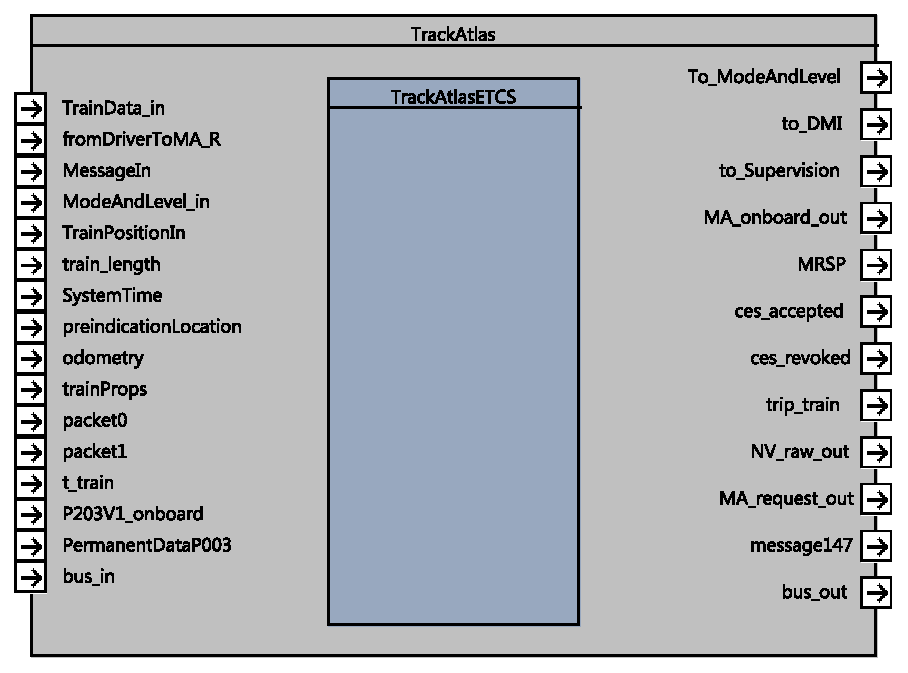
\includegraphics[width=.8\textwidth]{images/F2_4_TrackAtlas.pdf}
\caption{TrackAtlas component SysML diagram.}\label{f:manage_track_data_interface}
\end{figure}


\subsubsection{Inputs}\label{s:manage_track_data_inputs}

\paragraph{[Input 1 name]}

\begin{longtable}{p{.25\textwidth}p{.7\textwidth}}
\toprule
Input name				& [Name of the input] \\
\midrule
Description				& [Brief description of the input] \\
\midrule
Source					& [Name of the source component] \\ 
\midrule
Type					& [Type of the input] \\
\midrule
Valid range of values	& [Complete list of valid values] \\
\midrule
Behaviour when value is at boundary	& [Description of components behaviour when input value is at boundary] \\
\midrule
Behaviour for values out of valid range	& [Description of components behaviour when input value is out of valid range] \\
\midrule
Behaviour when value is erroneous, absent or unwanted (i.e. spurious) & [Description of components behaviour when value is erroneous, absent or unwanted (i.e. spurious)] \\
\bottomrule
\end{longtable}


\paragraph{[Input 2 name]}

\begin{longtable}{p{.25\textwidth}p{.7\textwidth}}
\toprule
Input name				& [Name of the input] \\
\midrule
Description				& [Brief description of the input] \\
\midrule
Source					& [Name of the source component] \\ 
\midrule
Type					& [Type of the input] \\
\midrule
Valid range of values	& [Complete list of valid values] \\
\midrule
Behaviour when value is at boundary	& [Description of components behaviour when input value is at boundary] \\
\midrule
Behaviour for values out of valid range	& [Description of components behaviour when input value is out of valid range] \\
\midrule
Behaviour when value is erroneous, absent or unwanted (i.e. spurious) & [Description of components behaviour when value is erroneous, absent or unwanted (i.e. spurious)] \\
\bottomrule
\end{longtable}


\subsubsection{Outputs}\label{s:manage_track_data_outputs}

\paragraph{[Output 1 name]}

\begin{longtable}{p{.25\textwidth}p{.7\textwidth}}
\toprule
Output name				& [Name of the output] \\
\midrule
Description				& [Brief description of the output] \\
\midrule
Destination				& [Name of the destination component(s)] \\ 
\midrule
Type					& [Type of the output] \\
\midrule
Valid range of values	& [Complete list of valid values] \\
\midrule
Behaviour when value is at boundary	& [Description of components behaviour when output value is at boundary] \\
\midrule
Behaviour for values out of valid range	& [Description of components behaviour when output value is out of valid range] \\
\midrule
Behaviour when value is erroneous, absent or unwanted (i.e. spurious) & [Description of components behaviour when value is erroneous, absent or unwanted (i.e. spurious)] \\
\bottomrule
\end{longtable}


\paragraph{[Output 2 name]}

\begin{longtable}{p{.25\textwidth}p{.7\textwidth}}
\toprule
Output name				& [Name of the output] \\
\midrule
Description				& [Brief description of the output] \\
\midrule
Destination				& [Name of the destination component(s)] \\ 
\midrule
Type					& [Type of the output] \\
\midrule
Valid range of values	& [Complete list of valid values] \\
\midrule
Behaviour when value is at boundary	& [Description of components behaviour when output value is at boundary] \\
\midrule
Behaviour for values out of valid range	& [Description of components behaviour when output value is out of valid range] \\
\midrule
Behaviour when value is erroneous, absent or unwanted (i.e. spurious) & [Description of components behaviour when value is erroneous, absent or unwanted (i.e. spurious)] \\
\bottomrule
\end{longtable}


\subsection{Subcomponents}\label{s:manage_track_data_subcomponents}

\subsubsection{StoreRaw\_NV}
%set the master document for easy compilation
%!TEX root = ../D3_5_3.tex

\paragraph{Component Requirements}

\begin{longtable}{p{.25\textwidth}p{.7\textwidth}}
\toprule
Component name			& StoreRaw\_NV \\
\midrule
Link to SCADE model		& {\footnotesize \url{https://github.com/openETCS/modeling/tree/master/model/Scade/
System/ObuFunctions/TrackAtlas/TA\_Storage}} \\
\midrule
SCADE designer			& Jakob G\"artner, LEA Railergy \\
\midrule
Description				& Receives National Values from the track. Stores them "as-is" onboard. If Subset\_026 chapter 6 is applicable, baseline 3 conformal information is calculated based on packet 3 and packet 203 (according to older versions). Missing trackside information is complemented throug default onboard values. \\
\midrule
Input documents	& 
Subset-026, Chapter 6
Subset-026, Chapter 7
Subset-026, Chapter 8\\
\midrule
Safety integrity level	& 4 \\
\midrule
Time constraints		& n/a \\
\midrule
API requirements 		& Based on data formats and functions defined by TrackMessages package\\
\bottomrule
\end{longtable}


\paragraph{Interface}

For an overview of the interface of this internal component we refer to the SCADE model (cf.~link above) respectively the SCADE generated documentation.

\subsubsection{Build\_GradientProfile}
%set the master document for easy compilation
%!TEX root = ../D3_5_3.tex

\paragraph{Component Requirements}

\begin{longtable}{p{.25\textwidth}p{.7\textwidth}}
\toprule
Component name			& Build\_GradientProfile \\
\midrule
Link to SCADE model		& {\footnotesize \url{https://github.com/openETCS/modeling/tree/master/model/Scade/
System/ObuFunctions/TrackAtlas/TA\_Gradient.xscade}} \\
\midrule
SCADE designer			& Jakob G\"artner, LEA Railergy  \\
\midrule
Description				& Receives Track to Train Packet 21 (Gradient Profile). References the data to the train coordinate system. Converts incremental distances to absolute distances in the train's coordinate system. Merges the information from sequentially received packets into a continuous Gradient Profile. Truncates the profile as required\\
\midrule
Input documents	& 
Subset-026, Chapter 3.11.12\newline
Subset-026, Chapter 7\\

\midrule
Safety integrity level	& 4 \\
\midrule
Time constraints		& n/a\\
\midrule
API requirements 		& n/a \\
\bottomrule
\end{longtable}


\paragraph{Interface}

For an overview of the interface of this internal component we refer to the SCADE model (cf.~link above) respectively the SCADE generated documentation.

\subsubsection{Build\_MA}
%set the master document for easy compilation
%!TEX root = ../D3_5_3.tex

\paragraph{Component Requirements}

\begin{longtable}{p{.25\textwidth}p{.7\textwidth}}
\toprule
Component name			& Build\_MA \\
\midrule
Link to SCADE model		& {\footnotesize \url{http://???}} \\
\midrule
SCADE designer			& Jakob G\"artner, LEA \\
\midrule
Description				& [Brief description of functionality] \\
\midrule
Input documents	& 
Subset-026, Chapter ?.?\newline
Subset-026, Chapter ?.?\newline
Subset-026, Chapter ?.?.?\\
\midrule
Safety integrity level	& 4 \\
\midrule
Time constraints		& [If applicable description of time constraints, otherwise n/a] \\
\midrule
API requirements 		& [If applicable description of API requirements, otherwise n/a] \\
\bottomrule
\end{longtable}


\paragraph{Interface}

For an overview of the interface of this internal component we refer to the SCADE model (cf.~link above) respectively the SCADE generated documentation.

\subsubsection{Build\_MRSP}
%set the master document for easy compilation
%!TEX root = ../D3_5_3.tex

\paragraph{Component Requirements}

\begin{longtable}{p{.25\textwidth}p{.7\textwidth}}
\toprule
Component name			& Build\_MRSP \\
\midrule
Link to SCADE model		& {\footnotesize \url{https://github.com/openETCS/modeling/tree/master/model/Scade/
System/ObuFunctions/TrackAtlas/TA\_MRSP}} \\
\midrule
SCADE designer			& Jakob G\"artner, LEA \\
\midrule
Description				& Reduces the various Speed Profiles to Most Restrictive Speed Profile information \\
\midrule
Input documents	& 
Subset-026, Chapter 3.11\\
\midrule
Safety integrity level	& 4 \\
\midrule
Time constraints		& n/a \\
\midrule
API requirements 		& n/a \\
\bottomrule
\end{longtable}


\paragraph{Interface}

For an overview of the interface of this internal component we refer to the SCADE model (cf.~link above) respectively the SCADE generated documentation.

\subsubsection{Manage\_EmergencyStop}
%set the master document for easy compilation
%!TEX root = ../D3_5_3.tex

\paragraph{Component Requirements}

\begin{longtable}{p{.25\textwidth}p{.7\textwidth}}
\toprule
Component name			& Manage\_EmergencyStop \\
\midrule
Link to SCADE model		& {\footnotesize \url{https://github.com/openETCS/modeling/tree/master/model/Scade/
System/ObuFunctions/TrackAtlas/TA\_EmergencyS_top.xscade}} \\
\midrule
SCADE designer			& Johannes Kastner, ICS AG; Jakob G\"artner, LEA Railergy\\
\midrule
Description				& Manages Emergency Stop Messages\\
\midrule
Input documents	& 
Subset-026, Chapter 3\\
\midrule
Safety integrity level	& 4 \\
\midrule
Time constraints		& n/a \\
\midrule
API requirements 		& n/a \\
\bottomrule
\end{longtable}


\paragraph{Interface}

For an overview of the interface of this internal component we refer to the SCADE model (cf.~link above) respectively the SCADE generated documentation.

\subsubsection{C\_P003V1\_OBU\_P003\_OBU}
%set the master document for easy compilation
%!TEX root = ../D3_5_3.tex

\paragraph{Component Requirements}

\begin{longtable}{p{.25\textwidth}p{.7\textwidth}}
\toprule
Component name			& C\_P003V1\_OBU\_P003\_OBU \\
\midrule
Link to SCADE model		& {\footnotesize \url{http://???}} \\
\midrule
SCADE designer			& Jakob G\"artner, LEA \\
\midrule
Description				& [Brief description of functionality] \\
\midrule
Input documents	& 
Subset-026, Chapter ?.?\newline
Subset-026, Chapter ?.?\newline
Subset-026, Chapter ?.?.?\\
\midrule
Safety integrity level	& 4 \\
\midrule
Time constraints		& [If applicable description of time constraints, otherwise n/a] \\
\midrule
API requirements 		& [If applicable description of API requirements, otherwise n/a] \\
\bottomrule
\end{longtable}


\paragraph{Interface}

For an overview of the interface of this internal component we refer to the SCADE model (cf.~link above) respectively the SCADE generated documentation.

\subsubsection{GradientProfile\_to\_DMI}
%set the master document for easy compilation
%!TEX root = ../D3_5_3.tex

\paragraph{Component Requirements}

\begin{longtable}{p{.25\textwidth}p{.7\textwidth}}
\toprule
Component name			& GradientProfile\_to\_DMI \\
\midrule
Link to SCADE model		& {\footnotesize \url{http://???}} \\
\midrule
SCADE designer			& Jakob G\"artner, LEA \\
\midrule
Description				& [Brief description of functionality] \\
\midrule
Input documents	& 
Subset-026, Chapter ?.?\newline
Subset-026, Chapter ?.?\newline
Subset-026, Chapter ?.?.?\\
\midrule
Safety integrity level	& 4 \\
\midrule
Time constraints		& [If applicable description of time constraints, otherwise n/a] \\
\midrule
API requirements 		& [If applicable description of API requirements, otherwise n/a] \\
\bottomrule
\end{longtable}


\paragraph{Interface}

For an overview of the interface of this internal component we refer to the SCADE model (cf.~link above) respectively the SCADE generated documentation.

\subsubsection{Manage\_MA\_Request}
%set the master document for easy compilation
%!TEX root = ../D3_5_3.tex

\paragraph{Component Requirements}

\begin{longtable}{p{.25\textwidth}p{.7\textwidth}}
\toprule
Component name			& Manage\_MA\_Request \\
\midrule
Link to SCADE model		& {\footnotesize \url{https://github.com/openETCS/modeling/tree/master/model/Scade/
System/ObuFunctions/TrackAtlas/TA\_MA\_Request}} \\
\midrule
SCADE designer			& Christian Stahl, TWT GmbH \\
\midrule
Description				& Manages reception of MA request parameters and sends MA request as specified\\
\midrule
Input documents	& 
Subset-026, Chapter ?.?\newline
Subset-026, Chapter ?.?\newline
Subset-026, Chapter ?.?.?\\
\midrule
Safety integrity level	& 4 \\
\midrule
Time constraints		& n/a \\
\midrule
API requirements 		& n/a]\\
\bottomrule
\end{longtable}


\paragraph{Interface}

For an overview of the interface of this internal component we refer to the SCADE model (cf.~link above) respectively the SCADE generated documentation.

\subsubsection{TA\_to\_ML}
%set the master document for easy compilation
%!TEX root = ../D3_5_3.tex

\paragraph{Component Requirements}

\begin{longtable}{p{.25\textwidth}p{.7\textwidth}}
\toprule
Component name			& TA\_to\_ML \\
\midrule
Link to SCADE model		& {\footnotesize \url{http://???}} \\
\midrule
SCADE designer			& Jakob G\"artner, LEA \\
\midrule
Description				& [Brief description of functionality] \\
\midrule
Input documents	& 
Subset-026, Chapter ?.?\newline
Subset-026, Chapter ?.?\newline
Subset-026, Chapter ?.?.?\\
\midrule
Safety integrity level	& 4 \\
\midrule
Time constraints		& [If applicable description of time constraints, otherwise n/a] \\
\midrule
API requirements 		& [If applicable description of API requirements, otherwise n/a] \\
\bottomrule
\end{longtable}


\paragraph{Interface}

For an overview of the interface of this internal component we refer to the SCADE model (cf.~link above) respectively the SCADE generated documentation.

\subsubsection{SSP\_to\_MRSP}
%set the master document for easy compilation
%!TEX root = ../D3_5_3.tex

\paragraph{Component Requirements}

\begin{longtable}{p{.25\textwidth}p{.7\textwidth}}
\toprule
Component name			& SSP\_to\_MRSP \\
\midrule
Link to SCADE model		& {\footnotesize \url{http://???}} \\
\midrule
SCADE designer			& Jakob G\"artner, LEA \\
\midrule
Description				& [Brief description of functionality] \\
\midrule
Input documents	& 
Subset-026, Chapter ?.?\newline
Subset-026, Chapter ?.?\newline
Subset-026, Chapter ?.?.?\\
\midrule
Safety integrity level	& 4 \\
\midrule
Time constraints		& [If applicable description of time constraints, otherwise n/a] \\
\midrule
API requirements 		& [If applicable description of API requirements, otherwise n/a] \\
\bottomrule
\end{longtable}


\paragraph{Interface}

For an overview of the interface of this internal component we refer to the SCADE model (cf.~link above) respectively the SCADE generated documentation.

\subsubsection{MRSP\_to\_MRSP\_to\_DMI}
%set the master document for easy compilation
%!TEX root = ../D3_5_3.tex

\paragraph{Component Requirements}

\begin{longtable}{p{.25\textwidth}p{.7\textwidth}}
\toprule
Component name			& MRSP\_to\_MRSP\_to\_DMI \\
\midrule
Link to SCADE model		& {\footnotesize \url{http://???}} \\
\midrule
SCADE designer			& Jakob G\"artner, LEA \\
\midrule
Description				& [Brief description of functionality] \\
\midrule
Input documents	& 
Subset-026, Chapter ?.?\newline
Subset-026, Chapter ?.?\newline
Subset-026, Chapter ?.?.?\\
\midrule
Safety integrity level	& 4 \\
\midrule
Time constraints		& [If applicable description of time constraints, otherwise n/a] \\
\midrule
API requirements 		& [If applicable description of API requirements, otherwise n/a] \\
\bottomrule
\end{longtable}


\paragraph{Interface}

For an overview of the interface of this internal component we refer to the SCADE model (cf.~link above) respectively the SCADE generated documentation.

